\documentclass[english,twoside, openright, hidelinks, 11 pt, class=report,crop=false]{standalone}
\input{../../preamb}



\begin{document}
{\Large Eksamen Matematikk 10. årstrinn våren 2023\hfill \\ {\footnotesize Løsning fra \color{blue} \href{https://sindreheggen.wordpress.com/}{OpenMathBooks prosjektet}}}	

\subsection*{Oppgave 1}
\textbf{Alternativ 1}\\
Vi setter
\[ \text{slikkepinne}=x\qquad,\qquad\text{sjokolade}=y \]
Da er
\begin{align}
	2x+2y &= 32 \label{opg1eq1}\vn
	4x+2y&= 44 \label{opg1eq2}
\end{align}
Ligning \eqref{opg1eq2} minus ligning \eqref{opg1eq1} gir at
\begin{align*}
	4x-2y-(2x+2y)&=44-32 \\
	2x&=12 \\
	x &= 6
\end{align*}
Av \eqref{opg1eq1} har vi da at
\begin{align*}
2\cdot2 +2y &= 32 \\
2y&=28 \\
y &= 14
\end{align*}
En slikepinne koster 6\enh{kr} og en sjokolade koster 14\enh{kr}. \vsk

\textbf{Alternativ 2}\\
Hvis vi i figuren til høyre i oppgaven tar bort det som er i figuren til venstre, har vi igjen to klubber som koster $44-32=12$\enh{kr}. Da koster en slikkepinne 6\enh{kr}. Skal to slikkepinner til 6\enh{kr} og to sjokolader koste 32\enh{kr} til sammen, må sjokoladen koste 14\enh{kr}.

\section*{Oppgave 2}
\abc{
\item  \begin{tabular}{c|c|c|c|}
	\hline
	FIGURNUMMER & 1 & 2 & 3 \\ \hline 
	TEGNING AV FIGUREN & 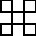
\includegraphics{opg2d1a} & 
\includegraphics{opg2d1b} & 
\includegraphics{opg2d1c} \\ \hline
	ANTALL BRIKKER 
	I FIGUREN & 5 & 12 & 21 \\ \hline
\end{tabular}
}


\end{document} 